% !TeX root = ../main.tex

\chapter{Réseau neuronal simple}

\section{Théorie}

\subsection{Le perceptron}

Le perceptron est le neurone le plus basique que l'on puisse trouver dans la
littérature. Un perceptron est défini par :
\begin{itemize}
\item $n$ entrées $x_i$
\item $1$ sortie $y$
\item $n$ poids $w_i$
\item $1$ biais $\theta$
\item $1$ fonction de composition $g : \mathbb{R}^n \to \mathbb{R}$
\item $1$ fonction d'activation $f : \mathbb{R} \to \mathbb{R}$
\end{itemize}

\begin{figure}[!ht]
\begin{center}
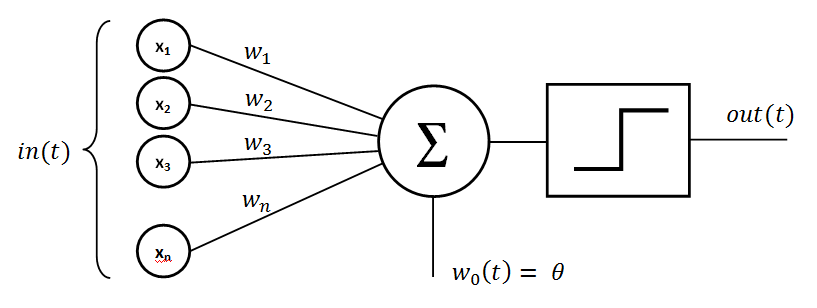
\includegraphics[scale=0.8]{images/perceptron.png}
\end{center}
\caption{Schéma d'un perceptron simple}
\end{figure}

\vspace{\parskip}
Sur sa construction, le perceptron est fortement inspiré sur le neurone humain,
sans pour autant en être une représentation réaliste.
Le perceptron détermine avec ses entrées si il "active" ou non la sortie, c'est
à dire s'il relaie le signal. Pour cela il rassemble toutes les données des
entrées $x_i$ à l'aide de la fonction de composition $g$. Le neurone ne donnant
pas la même importance à chaque entrée, on les pondère préalablement par les
poids notés $w_i$.
Finalement, on décide du signal de sortie à l'aide de la fonction d'activation
$f$. De base, le seuil d'activation est souvent centré en $0$. Pour palier à ce
problème, on prend également en entrée de la fonction d'activation un biais
$\theta$.

\medskip

En résumé, on a :
\[y = f(g(x_1w_1, x_2w_2, \ldots , x_nw_n) + \theta) \]

\medskip

Usuellement, la fonction d'activation est la somme :
\[y = f(\sum_{i=1}^n x_iw_i + \theta) \]

\medskip

On remarque que le biais agit comme le poids d'une entrée du neurone qui serait
toujours $1$.

\subsection{Le réseau}

Une réseau de neurones permet de créer des fonctions de bien plus grande
complexité qu'un simple neurone, permettant de résoudre des problèmes
jusqu'alors inaccessibles à la machine. Il permet par exemple de faire des
classifications sur le MNIST. Le MNIST est un problème classique où l'on a des
images représentant des chiffres manuscrits et pour lequel l'on doit déterminer
le chiffre représenté. C'est un problème d'une extrême simplicité pour un être
humain, mais presque impossible à résoudre avec une programmation classique
sans réseau neuronal. Ainsi, pour construire un réseau, chaque perceptron est
mis en relation avec ses pairs (un perceptron prend en entrée les sorties
d'autres perceptrons). On construit alors un graphe orienté dans lequel chaque
sommet est un perceptron. On se limitera dans un premier temps au cas d'un
réseau acyclique.

\bigskip

On peut définir plusieurs types de neurones dans un réseau :
\begin{itemize}
\item les neurones d'entrée
\item les neurones cachés
\item les neurones de sortie
\end{itemize}

\bigskip

Il faut donc autant de neurones d'entrée que de dimensions qu'a l'échantillon
que l'on veut soumettre au réseau. Par exemple dans le cadre du MNIST
on veut en entrée une image de dimension $28 \times 28$, on place donc $784$
neurones d'entrées. En pratique, les neurones d'entrée sont des neurones fictifs
; ils sont présents pour faciliter la construction du réseau de neurone.
En effet, ils ne sont soumis à aucun apprentissage et leur sortie est la même
que leur entrée. Nous ne les considérerons pas dans la théorie qui suit.

\medskip

Les neurones des couches cachées sont présents entre les neurones d'entrée et de
sortie. Ils sont utiles uniquement pour le calcul de la sortie. Le nombre de
couches et la taille des couches influent sur l'action du réseau. Un réseau à
multiples couches cachées sera capable de traiter des problèmes beaucoup plus
complexes qu'un réseau à simple couche cachée. Il est évident que cela augmente
néanmoins la complexité des calculs et le temps d'exécution.

\medskip

Les neurones de sortie sont ceux qui servent pour la classification de
l'échantillon d'entrée. Si l'on souhaite classifier une entrée il faut le même
nombre de neurones de sortie que de classes différentes possibles. Ainsi dans
l'exemple du MNIST, le but est de déterminer un chiffre donné sur une image.
Il y a donc $10$ possibilités (les 10 chiffres). Il y a donc $10$ neurones de
sortie.

\medskip

Par la suite, on appellera $\{x_i\}_{i \leq n}$ les entrées, $\{y_i\}_{i \leq m}$
 les sorties des neurones $\{y_i\}_{m+1-M \leq i \leq m}$ les sorties des
neurones de sorties, $\{\sigma_i\}_{i \leq m}$ les fonctions d'activations et
$\{\theta_i\}_{i \leq m}$ les biais.

\medskip

On définit enfin $\{F_i\}_{i \leq m}$ tel que $j \in E_i$ si et seulement si la
sortie du neurone $j$ est reliée au neurone $i$. On peut ainsi numéroter les
poids : $\{w_{ij}\}_{i \leq m, j \in F_i} $ le poids associé à l'entrée reliant
le neurone $j$ au neurone $i$.

\medskip

D'après ce qui précède, on obtient $\forall i \in [1, m]$ :

\[y_i = \sigma_i(\sum_{j \in F_i} y_jw_{ij} + \theta_i) \]

\subsection{Les réseaux à couche}

Il existe un type de réseau simplifié très utilisé. On partitionne l'ensemble
des neurones en $K$ ensembles. On chacun de ces ensembles une "couche". De plus,
chaque neurone d'une couche a comme entrées l'ensemble (ou partie) des sorties
des neurones de la couche précédente. On notera $\alpha^{(k)}_j$ l'élément $j$
de la couche $k$ de $\alpha$. On notera également $N_k$ le nombre de neuroneq à
la couche $k$. On a donc pour tout $k > 1$ :

\[y_i^{(k)} = \sigma_i^{(k)}(\sum_{j = 0}^{N_{k-1}} y_j^{(k-1)}w_{ij}^{(k)} + \theta_i^{(k)}) \]

On remarque que l'on peut simplifier la notation en considérant la formule
ci-dessus avec une approche vectorielle :

\[\overline{y^{(k)}} = w^{(k)} \times y^{(k-1)} + \theta^{(k)}\]
\[y^{(k)} = \sigma^{(k)}(\overline{y^{(k)}}) \]

On peut montrer que tout réseau acyclique peut se ramener à un réseau à couches
dont certains poids sont imposés comme nuls. Nous prenons donc l'hypothèse que
le réseau est un réseau à $K$ couches, que la première couche est l'ensemble des
 neurones d'entrée et la dernière couche l'ensemble des neurones de sortie, sans
 perte de généralité.

\subsection{L'apprentissage}

L'efficacité d'un réseau de neurones se mesure à la qualité de sa classification
. Celle-ci dépend des poids qui sont attribués à chacune de ses entrées. Il faut
donc déterminer la bonne combinaison de poids qui permettra au réseau de
simuler la fonction voulue. Le nombre de poids présents dans un réseau augmente
très rapidement et il devient complexe d'estimer cette bonne combinaison. Pour
cela, on procède à une phase apprentissage : on utilise un échantillon de
données dont on connaît le résultat pour construire un réseau avec les bon poids
. On part ainsi d'un réseau avec des poids aléatoires, choisis dans un
intervalle restreint et centré en zéro, et on les modifie en prenant en compte
les erreurs entre les valeurs obtenues et les valeurs théoriques. Dans la suite,
on s'intéressera à toute la démarche nécessaire pour arriver à cette
modification de poids.

\medskip

On notera $\{x_i\}_{i \leq n}$ et $\{Y_i\}_{i \leq M}$ les entrées et sorties
des échantillons.

\medskip

Pour déterminer les modifications à effectuer, on calcule la sortie du réseau de
 neurones à un échantillon de test donné et on mesure l'erreur. Pour cela,
on choisira une fonction qui mesurera la différence entre le vecteur de sortie
et le vecteur des sorties théoriques. Classiquement, on utilise la méthode des
moindres carrés $E_m$ ou bien une fonction softmax à laquelle on rajoute une
entropie croisée $E_s$:

\[E_m = \sum_{j = 1}^{M} \cfrac{(Y_j - y_j^{(K)})^2}{2}\]
\[E_s = \sum_{j = 1}^{M} Y_j \log \left(\cfrac{e^{y_j^{(K)}}}{\sum e^{y_i^{(K)}}}\right)\]

\subsection{La méthode des gradients}

On veut donc minimiser $E$ en modifiant les $w_{ij}$. Le problème ici est que
l'on a une connaissance limitée de $E$ en fonction des $w_{ij}$ car on ne
dispose des valeurs théoriques de sortie que pour un nombre fini de valeurs. Or
les méthodes de minimisation de fonctions reposent souvent sur une connaissance
continue de ce que l'on veut optimiser. La seule méthode viable est la méthode
des gradients.

\medskip

On a une fonction $f$, appelée fonction de coût, que l'on veut minimiser par
rapport à un facteur $x$. On crée alors une suite $(x_n)$ telle que
$x_{n+1} = x_{n} - \cfrac{\partial f}{\partial x}(x_n)$.
L'idée est se déplacer sur le potentiel de $f$ grâce à son gradient. Avec cette
méthode, on peut calculer facilement la suite $(x_n)$ car il suffit d'évaluer
le gradient en un point et non plus en un nombre continument infini.

\medskip

Cependant, cette méthode est imprécise et il arrive qu'elle converge vers un
minimum local. En pratique, l'ajout de neurones va augmenter le nombre de
dimensions du gradient et donc permettre de limiter le nombre de minima locaux.

\medskip

\subsection{La rétropropagation}

D'après ce qui précède, l'objectif est donc d'évaluer pour tout $w_{ij}^{(k)}$ :
 $\cfrac{\partial E}{\partial w_{ij}^{(k)}}$.

\begin{align*}
\cfrac{\partial E}{\partial w_{ij}^{(k)}} &= \sum_{l = 1}^{M} \cfrac{\partial y_l^{(K)}}{\partial w_{ij}^{(k)}} \times \cfrac{\partial E}{\partial y_l}\\
&= \left\langle\cfrac{\partial y^{(K)}}{\partial w_{ij}^{(k)}}, J_E\right\rangle\\
&= \left\langle\cfrac{\partial \overline{y^{(K)}}}{\partial w_{ij}^{(k)}} \odot \sigma'(\overline{y^{(K)}}), J_E\right\rangle \\
&= \left\langle\cfrac{\partial \overline{y^{(K)}}}{\partial w_{ij}^{(k)}} ,\sigma'(\overline{y^{(K)}}) \odot J_E\right\rangle
\end{align*}

Avec $J_E$ la jacobienne de $E$ au point considéré.
Calculons maintenant $\cfrac{\partial \overline{y^{(l)}}}{\partial w_{ij}^{(k)}}$.
Tout d'abord, remarquons que si $l = k$ alors on a simplement :

\[\cfrac{\partial \overline{y^{(k)}}}{\partial w_{ij}^{(k)}} = E_{ij} y^{(k-1)} = y^{(k-1)}_j e_i\]

Ceci vient du fait que le réseau étant acyclique, $ y^{(l)}$ ne dépend pas de
$w_{ij}^{(k)}$ pour $l < k$. De même, pour $l > k$, on obtient :

\begin{align*}
\cfrac{\partial \overline{y^{(l)}}}{\partial w_{ij}^{(k)}} &= w^{(l)} \times \cfrac{\partial y^{(l-1)}}{\partial w_{ij}^{(k)}}\\
&= w^{(l)} \times \left(\sigma(\overline{y^{(l-1)}}) \odot \cfrac{\partial \overline{y^{(l-1)}}}{\partial w_{ij}^{(k)}}\right)
\end{align*}

Donc en supposant qu'il existe un vecteur $v$ tel que $\cfrac{\partial E}{\partial w_{ij}^{(k)}} = \left\langle\cfrac{\partial \overline{y^{(l)}}}{\partial w_{ij}^{(k)}} ,v\right\rangle$ :

\begin{align*}
\cfrac{\partial E}{\partial w_{ij}^{(k)}} &= \left\langle w^{(l)} \times \left(\sigma(\overline{y^{(l-1)}}) \odot \cfrac{\partial \overline{y^{(l-1)}}}{\partial w_{ij}^{(k)}}\right) ,v\right\rangle\\
&= \left\langle\sigma(\overline{y^{(l-1)}}) \odot \cfrac{\partial \overline{y^{(l-1)}}}{\partial w_{ij}^{(k)}},{}^t \! w^{(l)} \times v\right\rangle\\
&= \left\langle\cfrac{\partial \overline{y^{(l-1)}}}{\partial w_{ij}^{(k)}},\sigma(\overline{y^{(l-1)}}) \odot ({}^t \! w^{(l)} \times v)\right\rangle\\
\end{align*}

Donc il existe $u = \sigma(\overline{y^{(l-1)}}) \odot ({}^t \! w^{(l)} \times v)$
tel que $\cfrac{\partial E}{\partial w_{ij}^{(k)}} = \left\langle\cfrac{\partial \overline{y^{(l-1)}}}{\partial w_{ij}^{(k)}} ,u\right\rangle$

Donc par récurrence, pour tout $l \geq k$ il existe $\delta y^{(l)}$ tel que :
\[\cfrac{\partial E}{\partial w_{ij}^{(k)}} = \left\langle\cfrac{\partial \overline{y^{(l)}}}{\partial w_{ij}^{(k)}} ,\delta y^{(l)}\right\rangle\]

On remarquera que $\delta y^{(l)}$ ne dépend pas de $w_{ij}^{(k)}$. On appellera
 $\delta y^{(l)}_j$ le gradient du neurone $j$ de la couche $l$. Ce gradient
 vérifie la relation de récurrence suivante d'après ce qui précède :

\[
\left \{
\begin{array}{c @{=} c}
    \delta y^{(K)} & \sigma'(\overline{y^{(K)}}) \odot J_E\\
    \delta y^{(k)} & \sigma(\overline{y^{(k)}}) \odot ({}^t \! w^{(k+1)} \times \delta y^{(k+1)})\\
\end{array}
\right.
\]

On a alors :

\begin{align*}
\cfrac{\partial E}{\partial w_{ij}^{(k)}} &= \left\langle\cfrac{\partial \overline{y^{(k)}}}{\partial w_{ij}^{(k)}} ,\delta y^{(k)}\right\rangle\\
&= \left\langle y^{(k-1)}_j e_i,\delta y^{(k)}\right\rangle\\
& = y^{(k-1)}_j \times \delta y^{(k)}_i
\end{align*}

Donc :

\[\Delta w^{(k)}_{ij} = \lambda \times y^{(k-1)}_j \times \delta y^{(k)}_i\]

\[\Delta w^{(k)} = \lambda \times (\delta y^{(k)} \times {}^t \! y^{(k-1)})\]

On obtient donc un algorithme d'apprentissage qui se fait en deux temps : tout
d'abord le calcul du gradient qui se fait récursivement, puis le calcul de la
différence de poids à appliquer. On remarque dans ce cas que l'on propage le
gradient de la fin du réseau vers le début. C'est ceci qui donne le nom à la
méthode employée : la rétropropagation.

\section{L'implémentation}

\subsection{Le neurone}

Le neurone est une classe, il a pour attributs :
\begin{itemize}
  \item le nombre de ses entrées (\verb+int+).
  \item les valeurs de ses entrées (\verb+vector<double>+).
  \item les poids qu'il leur attribue (\verb+vector<double>+).
  \item son biais (\verb+int+).
  \item sa fonction de composition (\verb+compositionFunction+).
  \item sa fonction d'activation (\verb+activationFunction+).
\end{itemize}

\medskip

Il dispose des méthodes suivantes :
\begin{itemize}
  \item \verb+description()+ : indique l'état du neurone.
  \item \verb+reset()+ : remet à zero ses entrées et sa sortie.
  \item les getters et les setters pour les poids, le nombre d'entrées, les
  fonctions de composition...
  \item \verb+calculateOutput()+ : calcul la sortie du neurone en fonction
  de ses entrées.
  \item \verb+getActivationDerivative+ : calcul de la dérivée de la fonction
  d'activation au point observé.
  \item \verb+getCompositionDerivative+ : idem pour la fonction de composition.
\end{itemize}

\subsection{Le réseau}

Le réseau est aussi implémenté en tant que classe.
Un réseau dispose :
\begin{itemize}
  \item d'un nom (\verb+string+).
  \item d'une date de création (\verb+string+).
  \item de ses neurones (\verb+vector<Neuron>+).
  \item de la liste de ses neurones d'entrée (\verb+vector<unsigned long>+).
  \item de la liste de ses neurones de sortie (\verb+vector<unsigned long>+).
  \item de la matrice des liens entre neurones (\verb+vector<vector<double>>+).
  \item de son facteur d'apprentissage (\verb+unsigned long+).
  \item de ses valeurs en entrée (\verb+vector<double>+).
  \item de la matrice des sorties des neurones (\verb+vector<double>+).
\end{itemize}

\medskip

Il dispose des méthodes nécessaires à la propagation du signal ainsi qu'à
sa rétropropagation.

\subsection{Améliorations apportées}

Nous avons ensuite amélioré le code pour diminuer le temps de calcul et clarfier
la structure. Les éléments à améliorer sont :
\begin{itemize}
\item La structure orientée objet
\item Le single-threading
\item calcul à chaque pas des sorties de chaque neurone
\end{itemize}

\medskip

Nous nous sommes progressivement débarrassés de la structure d'objet du neurone
en effectuant les conversions suivantes :

\medskip

\begin{tabular}{c|c}
   structure objet & nouvelle structure \\
   \hline
   neurones.poids + matrice des poids + matrice des relations & matrice des poids \\
   neuron.activationFunction & vecteur de fonctions d'activation \\
   neuron.compositionFunction & on ne considère plus que la somme \\
   neuron.inputs/output & vecteur des entrées/sorties de tout le réseau \\
   neuron.bias & vecteur des biais de chaque neurone du réseau \\
   dérivée de la fonction de composition & vaut 1
\end{tabular}

\medskip

De plus, nous avons déterminé en amont les neurones voisins qui nécessitaient
un rafraîchissement de leur sortie. Cela permet de ne pas calculer à chaque
itération la sortie de tous les neurones du réseau. Lors de la création du
réseau est construite une liste de vecteurs des neurones dont il faut évaluer
la sortie au tour $i$.

\section{Résultats}

Après une longue période de débogage, nous avons obtenu des résultats
satisfaisants.

%TODO

\subsection{Le XOR}

%TODO

\subsection{Le MNIST}

Les données du problème du MNIST sont réparties en deux fichiers :
\begin{itemize}
    \item Le set d'apprentissage qui contient 60000 entrées (images de 784 pixels
          des chiffres manuscrits suivis des données des chiffres représentés)
    \item Le set de test qui contient 10000 entrées (différentes de celle du set
          d'apprentissage)
\end{itemize}

\medskip

Les valeurs des entrées sont stockées dans les fichiers entre 0 et 255, nous
les avons centrées et normalisées (entre $-0.5$ et $0.5$).

\medskip

Tous les résultats présentés par la suite sont établis en soumettant au réseau
après apprentissage les 10000 entrées du set de test et en comparant la sortie
attendue et la sortie obtenue. On obtient le résultat du calcul du réseau en
prenant la sortie du réseau avec la valeur maximale.

\subsubsection{Le classificateur linéaire}

En créant un réseau neuronal sans bias ni couche cachées on obtient un
classificateur linéaire. Les 10 neurones de sortie sont reliés chacun aux 784
neurones d'entrées. Les poids sont initialisés aléatoirement entre -1 et 1 selon
 une loi uniforme. La fonction d'activation est une siogmoïde, la composition
est une somme pondérée, et la fonction de coût est l'écart quadratique. Le
facteur d'apprentissage $\lambda$ est fixé à $0.3$ en accord avec la littérature
 sur le sujet.


\medskip

Les résultats d'un tel réseau sont forts intéressants car permettent après un
apprentissage stochastique des 60000 échantillons de test d'obtenir un
pourcentage moyen d'erreur de XX \%. (Moyenne effectuée sur 100 réalisations).

%TODO

\subsubsection{Réseau sans couche cachées}

\subsection{Réseau avec 1 couche cachée}

\subsubsection{Réseau avec deux couches cachées}
